\section{Software}
\label{section:software}

This section describes the software used in this work. Two different applications were developed. One application was the software that constitutes the mobile 3D scanner, which was developed in a framework called Robot Operating System, described in \cref{section:ros}. The other one is the software used to process the data recorded by the 3D scanner, which is described in \cref{section:processing-application}.

\subsection{Robot Operating System}
\label{section:ros}

Robot Operating System, or ROS, is a software architecture for robot development, providing a collection of tools, libraries and conventions to simplify the development of complex robotic systems. It was originally created at stanford University in the mid-2000s and new is widely adopted as the standard framework for robotics by most research communities.

Its design principles follow the one of a distributed system. In ROS, a system is composed by multiple nodes that have just one task and communicate between them by message passing. To achieve this, ROS, in its core, has the infrastructure responsible for the:

\begin{description}
    \item[Orchestration]. ROS runs, stops and monitors all nodes, so in the case of failure, for example, ROS is capable of restarting the node.
    \item[Communication]. ROS provides both the pipelining to distribute messages as well as the standard serialization specification.
    \item[Configuration]. ROS provides a key-value store for parameters that are accessible for nodes. These parameters can be specified when the node is created and also changed dynamically at runtime.
    \item[Discovery]. Each node in the environment can inspect it, such as finding other nodes and finding topics.
\end{description}

This architecture has many advantages, such as:

\begin{description}
    \item[Fault-tolerant]. A failure in one node does not affect other nodes, so there is not a overall system crash, unlike monolithic systems. Usually, because errors are transitive and not very frequent, a restart-on-failure policy is used to keep the downtime low.
    \item[More generic]. Because each node has a single responsibility, they tend to be more generic and detached to a single project, so integration in a new project can be easy. This is fundamental to reduce the need to "reinvent the wheel", therefore reducing the development cost and time of this complex systems.
    \item[Easier to develop]. Each component can be developed be separate developers, with different languages and independent release cycles, because they do not have any dependency between each over and only a message specification needs to be agreed on between developer teams, making collaborative development possible. Debugging is also easier, because each node can be unit-tested separated from the "real environment".
    \item[Large Community]. ROS is open source, which incentivises different research groups to share packages. Also, ROS is widely adopted so multiple packages for numerous tasks are already programmed, and can be integrated easily into new systems. One of this examples are drivers, which almost never require to be developed, because most robotic hardware already has a developed driver.
\end{description}

ROS is split into 3 levels, according to~\cite{fernandez15}: the \textit{filesystem} level, the \textit{the computational graph} level and the \textit{community} level. Each level is composed of several core components, that make the whole system work, as seen in \cref{figure:ros_overview}. Some components that were required for this work are explained next.

\begin{figure}[h]
    \label{figure:ros_overview}
        
        \caption{ROS architecture overview}
    
        \tikzstyle{ros_level}=[rectangle, draw, text centered, thick, text width=8em, rounded corners, font=\bfseries]
        \tikzstyle{level}=[rectangle, draw, font=\bfseries, thick, rounded corners, inner xsep=0.5cm]
        \tikzstyle{component}=[rectangle, draw, text width=9em]
    
    
        \centering
        \begin{tikzpicture}[scale=0.9]
            
            \node[ros_level] (ROS) {ROS};
            \coordinate[below=0.4cm of ROS] (aux_node1);
            \node[level, below=0.6cm of aux_node1] (computational_graph) {Computational Graph};
            \node[level, left=1.7cm of computational_graph] (filesystem) {Filesystem};
            \node[level, right=1cm of computational_graph] (community) {Community};
    
            \draw[->] (ROS) -- (aux_node1) -- (computational_graph.north);
            \draw[->] (ROS) -- (aux_node1) -| (filesystem.north);
            \draw[->] (ROS) -- (aux_node1) -| (community);
    
            \coordinate[below=of filesystem.west, xshift=0.5cm] (aux_node2);
            \coordinate[below=of computational_graph.west, xshift=0.5cm] (aux_node3);
            \coordinate[below=of community.west, xshift=0.5cm] (aux_node4);
    
            \node[component, anchor=west, yshift=0cm] (meta_packages) at (aux_node2) {Meta Packages};
            \node[component, anchor=west, yshift=-0.8cm] (packages) at (aux_node2) {Packages};
            \draw[->] (filesystem.west) -- ++(-0.2cm, 0) |- (meta_packages.west);
            \draw[->] (filesystem.west) -- ++(-0.2cm, 0) |- (packages.west);
    
            \node[component, anchor=west, yshift=0cm] (nodes) at (aux_node3) {Nodes};
            \node[component, anchor=west, yshift=-0.8cm] (master) at (aux_node3) {Master};
            \node[component, anchor=west, yshift=-1.6cm] (param_server) at (aux_node3) {Parameter Server};
            \node[component, anchor=west, yshift=-2.4cm] (messages) at (aux_node3) {Messages};
            \node[component, anchor=west, yshift=-3.2cm] (topics) at (aux_node3) {Topics};
            \node[component, anchor=west, yshift=-4.0cm] (services) at (aux_node3) {Services};
            \node[component, anchor=west, yshift=-4.8cm] (bags) at (aux_node3) {Bags};
            \draw[->] (computational_graph.west) -- ++(-0.2cm, 0) |- (nodes.west);
            \draw[->] (computational_graph.west) -- ++(-0.2cm, 0) |- (master.west);
            \draw[->] (computational_graph.west) -- ++(-0.2cm, 0) |- (param_server.west);
            \draw[->] (computational_graph.west) -- ++(-0.2cm, 0) |- (messages.west);
            \draw[->] (computational_graph.west) -- ++(-0.2cm, 0) |- (topics.west);
            \draw[->] (computational_graph.west) -- ++(-0.2cm, 0) |- (services.west);
            \draw[->] (computational_graph.west) -- ++(-0.2cm, 0) |- (bags.west);
    
            \node[component, anchor=west, yshift=0cm] (distributions) at (aux_node4) {Distributions};
            \node[component, anchor=west, yshift=-0.8cm] (repositories) at (aux_node4) {Repositories};
            \node[component, anchor=west, yshift=-1.6cm] (ros_wiki) at (aux_node4) {ROS Wiki};
            \node[component, anchor=west, yshift=-2.4cm] (bug_ticket_system) at (aux_node4) {Bug Ticket System};
            \node[component, anchor=west, yshift=-3.2cm] (mailing_lists) at (aux_node4) {Mailing Lists};
            \node[component, anchor=west, yshift=-4.0cm] (ros_answers) at (aux_node4) {Ros Answers};
            \node[component, anchor=west, yshift=-4.8cm] (blog) at (aux_node4) {Blog};
            \draw[->] (community.west) -- ++(-0.2cm, 0) |- (distributions.west);
            \draw[->] (community.west) -- ++(-0.2cm, 0) |- (repositories.west);
            \draw[->] (community.west) -- ++(-0.2cm, 0) |- (ros_wiki.west);
            \draw[->] (community.west) -- ++(-0.2cm, 0) |- (bug_ticket_system.west);
            \draw[->] (community.west) -- ++(-0.2cm, 0) |- (mailing_lists.west);
            \draw[->] (community.west) -- ++(-0.2cm, 0) |- (ros_answers.west);
            \draw[->] (community.west) -- ++(-0.2cm, 0) |- (blog.west);
    
        \end{tikzpicture}
    
    \end{figure}

\subsubsection{Messages}

Messages are the communication element and are just structures of data composed by primitive types such as integers, floating point numbers, strings and other messages. All messages follows a schema, which is required to encode and decode the message. Messages are serialized in a binary format before and after the exchange, so messages are small and efficient. Moreover, all messages have a header, which contains a timestamp and the source of the message. 

\subsubsection{Topics}

Topics are named buses over which nodes exchange messages. Topics follow the publisher/subscriber paradigm, so nodes can both subscribe to receive messages or publish messages to the topics. The exchange of data is done anonymously, so nodes are not aware which nodes are publishing or subscribing to a topic. This way of exchanging data is well suited for streaming data, such as sensor data.

\subsubsection{Launch Files}

Launch files are xml files that describe the steps to launch multiple node, as well as setting parameters. Launch files also support composition, so a launch file can invoque other launch files. Launch files were used in this project extensively, to launch the drivers of the mobile robot and to launch the acquisitions.

\subsubsection{Bags}

A bag is a file format for storing ROS messages, and have a myriad of tools to store, process, visualize and analyze them. During runtime, bags can be used to store the messages published in multiple topics, so data can be analysed later. Also, messages in bag files can be republished back into the system for testing or visualization purposes.

In this work, bag files played a very important role, as they were responsible to store the sensor data and also the transformation graph of the 3D scanner.

\subsubsection{RViz}

RViz is a 3D visualizer for ROS for displaying sensor data, like laser scans and point clouds, and the representation of the robot state, like the position of the coordinate frames and the joints. RViz can be a indispensable debug tool, for example, by comparing the real environment with the displayed environment shown in RViz.

\subsubsection{TF}

TF is a package that keeps track of multiple coordinate frames and maintains the relationship between coordinate frames in a tree structure, called the transformation graph. This transformation graph can be queried to obtain the transformation between two frames at any point in time. Also, tf can work in distributed systems, just like ROS, so any node can publish transformations and the transformations can be obtained in any node. TF is also responsible to interpolate between the discrete transformations and handle transformations with different sampling rates.

\subsubsection{URDF}

Unified Robot Description Format, or URDF, is a format to represent a robot model, like the joints and links configuration and the geometry of the joints. This file is loaded at runtime and the transformations are published according to the joint state. 


\subsection{Processing Application}
\label{section:processing-application}

This application required a wide spectrum of libraries, frameworks, file formats and graphical programs, which are described next.

\subsubsection{Libraries and Frameworks}

The software developed in this work that implements the processing algorithms was done using the Python programming language and some libraries to provide both data structures and common algorithms. Both the language and libraries are described next.

\begin{description}
    \item[Python] is a general purpose programming language that become popular for its syntax and small learning curve. It is also the defacto language for science, along with MATLAB. However, inlike MATLAB, it is s open source, has large community and has plenty of libraries that provide many algorithms and efficient data structures. Also, it is a dynamic language, which facilitates the process of testing and debugging the code developed.

    \item[Numpy] is a library that contains an implementation of $nd$-arrays, as well as algorithms to manipulate them. This library was fundamental for this work to store and process the point data. The main advantage of this library is that it is implemented in compiled languages like C and Fortran to implement high performance and optimized data structures and algorithms, available through a clean interface in Python.

    \item[Pandas] is a library that provides a fundamental data structure which was extensively used in this work: the DataFrame. DataFrames store data in columns, which is perfect to store tabular data. This is a common way to store point information, because point clouds are, fundamentally, tables, where each property are stored as a column, like $x$, $y$, $z$ for position and $r$, $g$, $b$ for color. Also, because it relies on numpy arrays to store the data, it is still very high performance.

    \item[PIL], or Python Image Library, is a library for image loading and manipulation, and was used to read and write the images recorded by the camera. 
    
    \item[Jupyter] provides an interactive interfaces, called Jupyter notebooks, which provides interactive documents with embedded code. This notebooks are extremely useful and were used to document and explore the code that was used in this work.

\end{description}

\subsubsection{File Formats}

\begin{description}
    
    \item[AVRO] is a binary data serialization format that is user to store collections of structured data. This format was chosen to store the laserscans and the image metadata. AVRO relies on schemas, which describe the data in the file is stored with the data. Therefore, an AVRO file is self-describing and data can be read and write without much overhead. Moreover, this format is implemented in Python and has numerous tools for inspection and conversion of the data.

    \item[PLY], or Polygon File Format is one of the most used and supported file formats to store three dimensional data, like point clouds and meshes. It was originally developed and used in the Stanford University to store data from 3D scanners. It supports a wide number of properties, like color, transparency, surface normals and texture coordinates. It also supports the storage of custom properties, which were required for this work, for example in the segmentation for the calibration. Moreover, it supports binary encoding, so files are small and fast to read and write.

    \item[JPEG] is a commonly used format for images and was used to store the recorded images.

    \item[YAML] is an human readable format that was used to store the parameters of the acquisitions, suck as the the extrinsic calibration of the sensors. The advantage of this format is that files are very easy to read and modify by the user.

\end{description}

\subsubsection{Graphical Software}

\begin{description}
    
    \item[CloudCompare] is a software to render, process and manipulate 3d point clouds. It includes many algorithms, like point cloud registration, re-sampling, handling scalar fields, and automatic or interactive segmentation. It can also render point clouds using different shaders and support point cloud decimation, which is a technique that allows manipulation of large point clouds without a decrease in performance. A screenshot of this software can be seen in \cref{fig:cloud-compare}.

\end{description}

\begin{figure}[h]
    \centering
    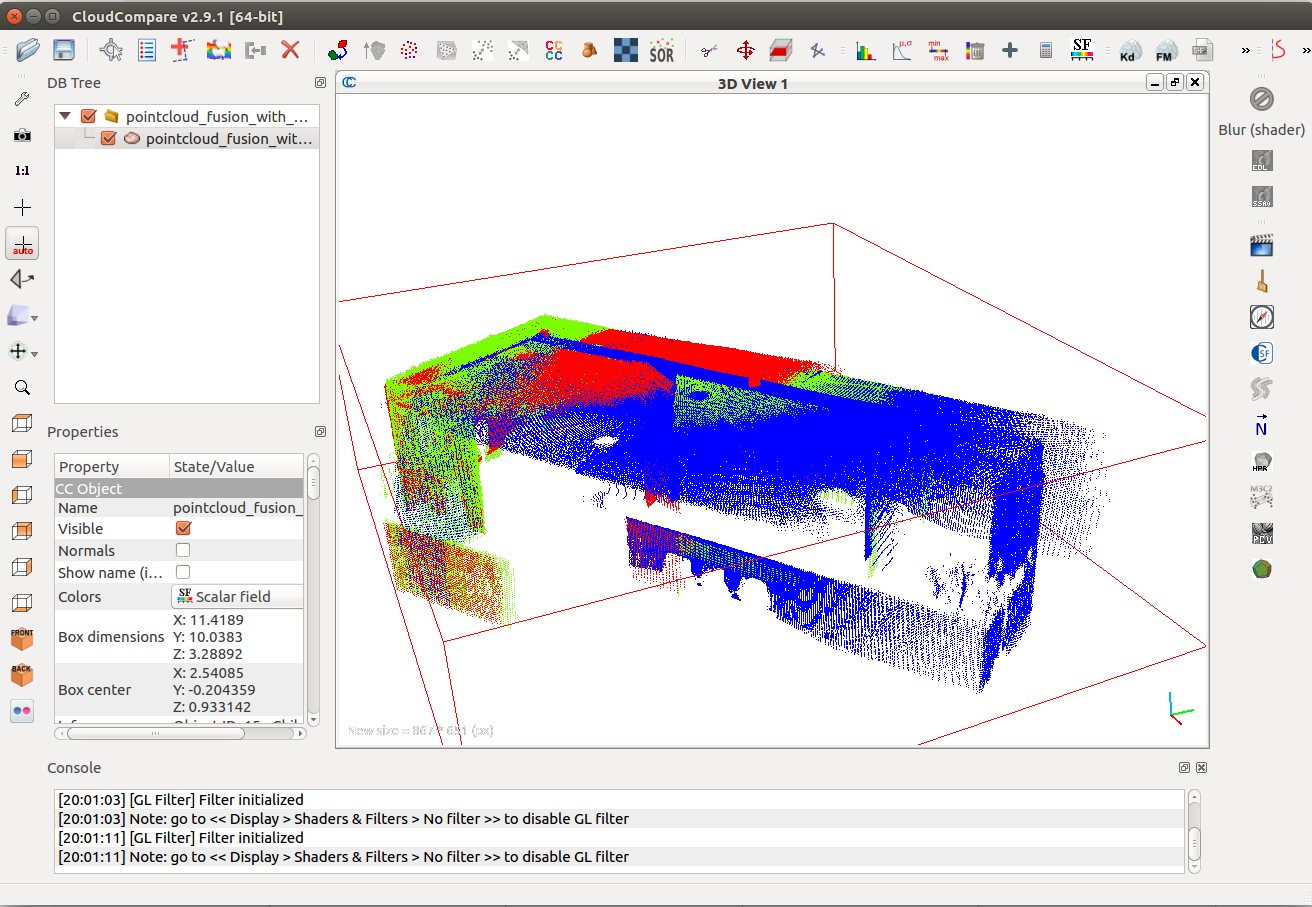
\includegraphics[width=15cm]{cloudcompare}
    \caption{Cloud Compare screenshot.}
    \label{fig:cloud-compare}
\end{figure}